
\lhead[\chaptername~\thechapter]{\rightmark}


\rhead[\leftmark]{}


\lfoot[\thepage]{}


\cfoot{}


\rfoot[]{\thepage}


\chapter{Ergebnisse und Diskussion}

\begin{figure}
	\centering
	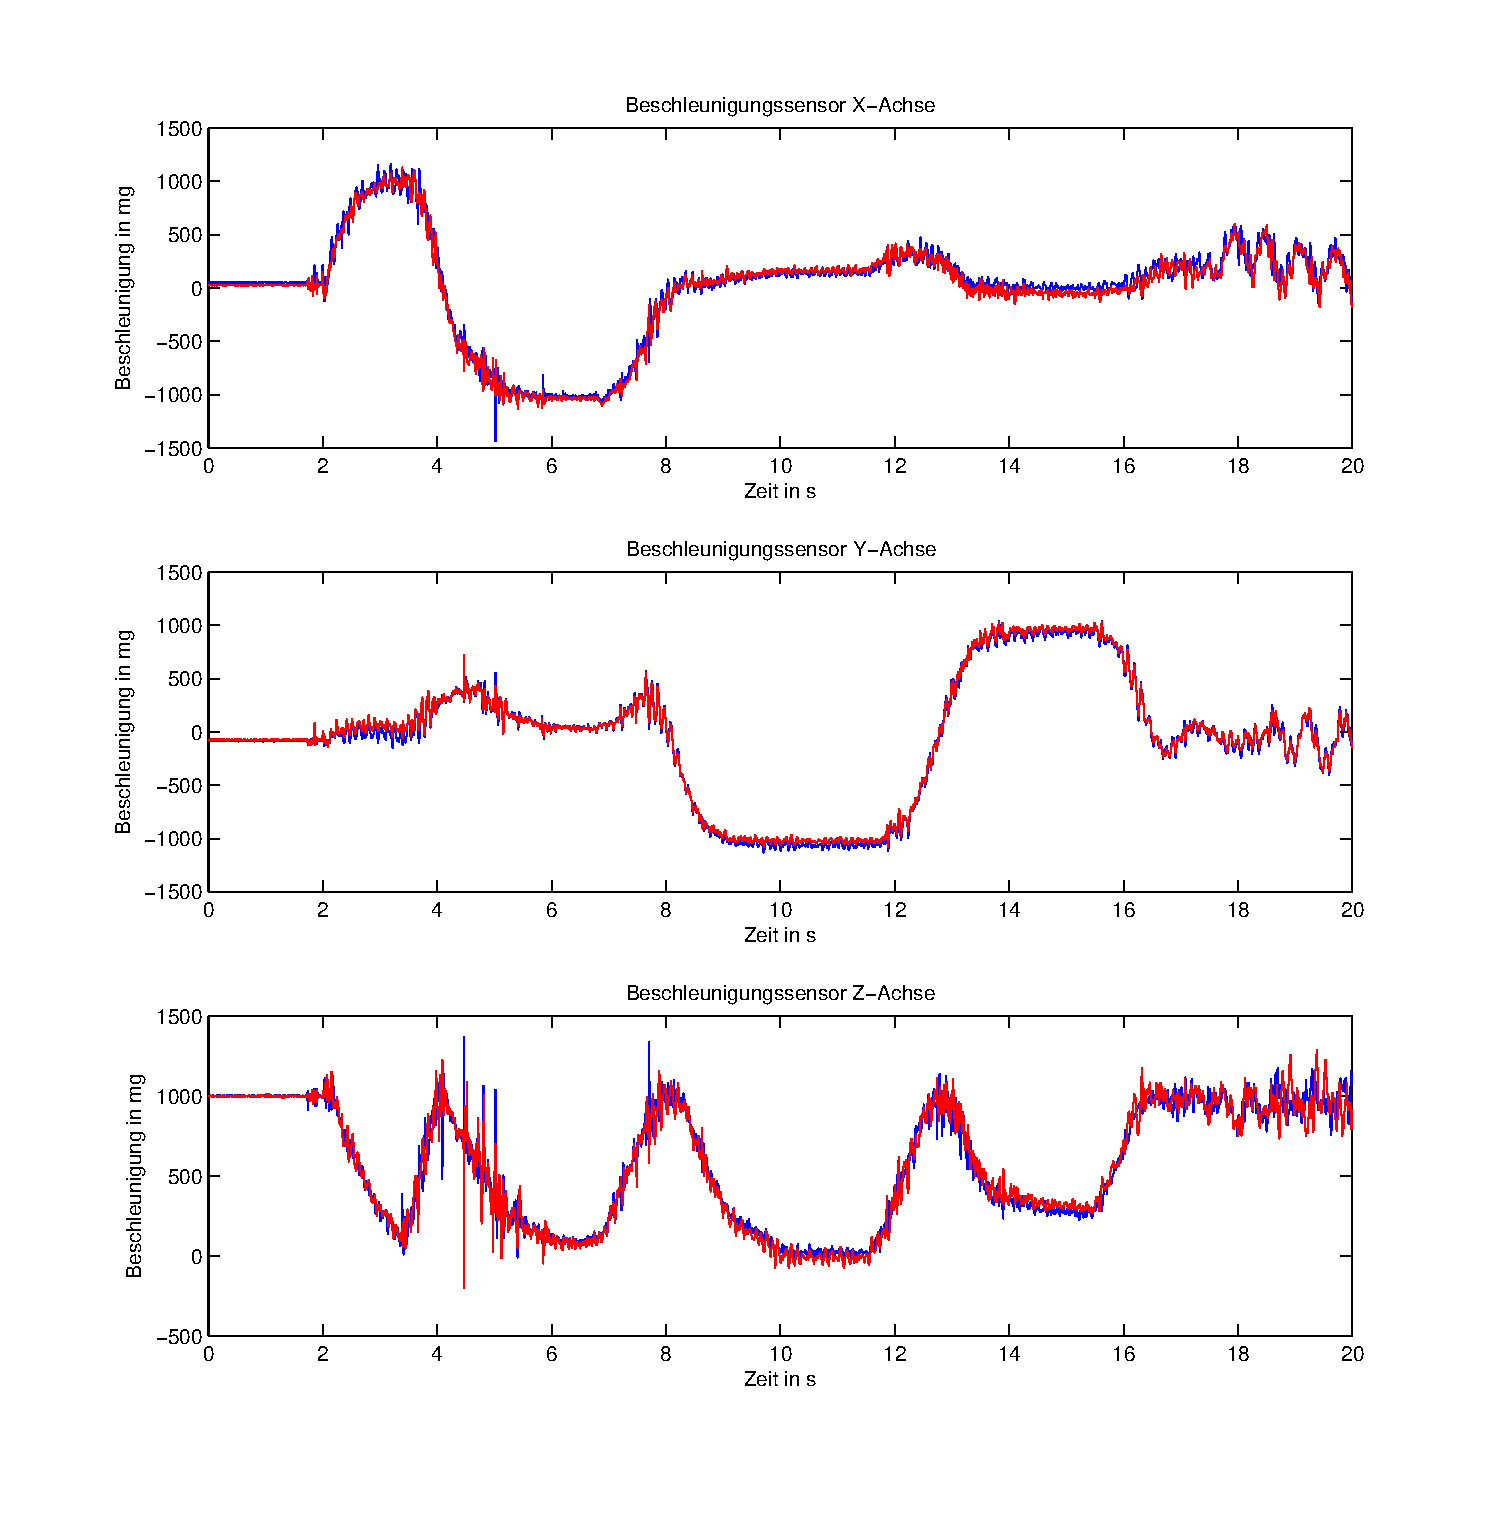
\includegraphics[width=1\textwidth]{images/Messergebnisse/calibration-wood-accel}
	\caption{Kalibrierung mit Holzgestell, Beschleunigungssensor.}
\end{figure}

\begin{figure}
	\centering
	\includegraphics[width=1\textwidth]{images/Messergebnisse/calibration-wood-gyro}
	\caption{Kalibrierung mit Holzgestell, Drehratensensor.}
\end{figure}

\begin{figure}
	\centering
	\includegraphics[width=1\textwidth]{images/Messergebnisse/calibration-wood-comparison}
	\caption{Kalibrierung Vergleich mit ABBA (Optimizer).}
\end{figure}

\begin{figure}
	\centering
	\includegraphics[width=1\textwidth]{images/Messergebnisse/calibration-faisal-move-accel}
	\caption{Kalibrierung mit Faisal, Beschleunigungssensor.}
\end{figure}

\begin{figure}
	\centering
	\includegraphics[width=1\textwidth]{images/Messergebnisse/calibration-faisal-move-gyro}
	\caption{Kalibrierung mit Faisal, Drehratensensor.}
\end{figure}

\begin{figure}
	\centering
	\includegraphics[width=1\textwidth]{images/Messergebnisse/calibration-faisal-chest-accel}
	\caption{Kalibrierung mit Faisal, Beschleunigungssensor, Bustatmung.}
\end{figure}

\begin{figure}
	\centering
	\includegraphics[width=1\textwidth]{images/Messergebnisse/calibration-faisal-chest-gyro}
	\caption{Kalibrierung mit Faisal, Drehratensensor, Brustatmung.}
\end{figure}

\begin{figure}
	\centering
	\includegraphics[width=1\textwidth]{images/Messergebnisse/calibration-faisal-tummy-accel}
	\caption{Kalibrierung mit Faisal, Beschleunigungssensor, Bauchatmung.}
\end{figure}

\begin{figure}
	\centering
	\includegraphics[width=1\textwidth]{images/Messergebnisse/calibration-faisal-tummy-gyro}
	\caption{Kalibrierung mit Faisal, Drehratensensor, Bauchatmung.}
\end{figure}

